\section{Quantum Pirate Game}
\label{sec:quantum_pirate}

\subsection{Hypothesis}
\label{subsec:qhipothesis}

The original Pirate Game is posed from the point of view of the captain. How should she allocate the treasure to the crew in order to maximize her payoff.
We can find the a equilibrium to the original Pirates Game and, while the solution may seem unexpected at first sight, it is fully described using backwards induction. 

When modelling this problem from a quantum theory perspective we are faced with some questions. The main difference from the original problem will rely on how the system is set up. Will the initial conditions provide different equilibria? Is there a condition where we are left with the classical problem? Is it possible for a captain, in a situation where we have more than two pirates left, to acquire all the coins?

We propose to study this problem for the $2$ and $3$ player games and trying to extrapolate for $N$ players. We will analyse the role of entanglement and superposition in the game system. Another aspect worth studying is the variation in the coin distribution on the payoff functions for the players.



\subsection{Quantum Model}
\label{subsec:description_2}

In order to model the problem we will start by defining it using the definition of quantum game ($\Gamma$), referred in \ref{eq:quantum_game_six_tuple}, Section \ref{sec:background_quantum_game_theory}\cite{Fra2011a}.

We want to keep the problem as close to the original as possible in order to better compare the results. Thus we will analyse the game from the point of view of the captain. Will her best response change?

In terms of mechanics and steps, this problem could be described using $3$ players and later extended to any number $N$ of players. 

We begin by assigning an offset to each pirate (in order to identify her), as in the Section \label{subsec:description}. The captain is number $1$ and the lower the number the higher the rank. 



\subsubsection{Game system: Setting up the Initial State}
\label{subsec:pirates_initialstate}

A game $\Gamma$ can be viewed as a system composed by qubits manipulated by players. In a $3$ player game there will be $3$ qubits, each manipulated by a different player. 

With $3$ players our system with be represented in a $\mathcal{H}^{8}$ using a state $\psi$. This means that to represent our system we will need vectors $2^{3}\times 1$ vectors, our system grows exponentialy with the number of players/qubits. Each pure basis $\mathcal{B}= \{ \vert 000\rangle , \vert 001\rangle , \vert 010\rangle , \vert 011\rangle , \vert 100\rangle , \vert 101\rangle , \vert 110\rangle , \vert 111\rangle \}$ of $\mathcal{H}^{8}$ will represent a possible outcome in the game. We assign a pure basis as $\vert 0\rangle = \vert C\rangle$ (``C'' from ``Cooperate''), and $\vert 1\rangle = \vert D\rangle$ (``D'' from ``Defect'').

For 200 players (for example), this game would be impractical to simulate in a classical computer. In this regard a quantum computer may enhance our power to simulate this kinds of experiments \cite{Rieffel2011}.

\begin{figure}[h]
\centering 
\includegraphics[scale=0.55]{Figures/architecture/GameTree/Slide1.png}
\caption{Game tree representation of the game ($3$ player). Red circles represent failed proposals, green represent accepted proposals. }
\label{fig:pg_architecturegametree}
\end{figure}

The initial system ($\vert \psi_{0}(\gamma) \rangle$), will be set up by defining an entanglement coefficient $\gamma$, that affect the way the three qubits (belonging to the three pirate players), are related \ref{eq:estado_inicial_pg}. 
We will entangle our state by applying the gate $\mathcal{J}$ \cite{Letters2002}. The parameter $\gamma$ becomes a way to measure the entanglement in the system\cite{Eisert2008}.

The index $0$ represents the depth of the game tree which can be examined in Figure \ref{fig:pg_architecturegametree}.

Due to the nature of quantum mechanics we have to pay attention to some details whe setting up our architecture. For example we cannot copy or clone unkown quantum states\cite{Rieffel2011}. 

The concept of entanglement is crucial to explain some phenomena in Quantum Mechanics (Section \ref{subsec:entanglement}). Analysing the role of entanglement in the system is also considered to be a major source of different results from the traditional Game Theory approach\cite{Fra2011a}\cite{Fra2011}\cite{Letters2002}\cite{Khan2011}\cite{Ricketts2006}. 


\begin{equation}
\label{eq:matrix_exponencial_esoterica}
\mathcal{J}=exp\left\{ i\frac{\gamma}{2}\left[\begin{array}{cc}
0 & 1\\
1 & 0
\end{array}\right]\otimes\left[\begin{array}{cc}
0 & 1\\
1 & 0
\end{array}\right]
\otimes\left[\begin{array}{cc}
0 & 1\\
1 & 0
\end{array}\right]
\right\}
\end{equation} 

\begin{equation}
\label{eq:estado_inicial_pg}
%\vert \psi_{0}(\gamma) \rangle= cos( \frac{\gamma}{2})\vert 00\rangle+ isin(\frac{\gamma}{2})\vert 11 \rangle, \gamma \in (0,\pi)
\begin{split}
\vert\psi_{in}(\gamma)\rangle=exp\left\{ i\frac{\gamma}{2}\left[\begin{array}{cc}
0 & 1\\
1 & 0
\end{array}\right]\otimes\left[\begin{array}{cc}
0 & 1\\
1 & 0
\end{array}\right]\otimes\left[\begin{array}{cc}
0 & 1\\
1 & 0
\end{array}\right]\right\} \vert000\rangle \\
=cos(\frac{\gamma}{2})\vert000\rangle+isin(\frac{\gamma}{2})\vert111\rangle,\gamma\in(0,\pi)
\end{split}
\end{equation}



\subsubsection{Strategic Space}
\label{subsec:strategic_space}

In Equation \ref{eq:quantum_game_six_tuple} there is the notion of a subset of unitary operators that the players can use to manipulate their assigned qubits. 

Each player will be able to manipulate a qubit in the system, in this case $\vert\varphi_{1}\rangle,\:\vert\varphi_{2}\rangle,$ and $\vert\varphi_{3}\rangle$, with one of two operators shown in Equation \ref{eq:operators_piratas_quanticos}. 

An operator is an unitary $2\times2$ matrix that is used to manipulate a qubit in the system.
This restriction of the strategic space is relevant to keep the problem as close to the classical version as possible. The two operators will correspond to the action of voting ``Yes'' or to Cooperate, and voting ``No'', meaning that they will not accept the proposal.  

The cooperation operator will be represented by the Identity operator ($o_{i0}$, where i identifies the qubit upon which player i will act). When assigned to a qubit this operator will leave it unchanged. 

The defection operator ($D$), will be represented by one of Pauli's Operators - the Bit-flip operator. This operator was chosen because it performs the classical operation NOT on a qubit.

These operators are also permutation matrices, so our players are in fact permutating the state of their qubit as in the roullete quantum model (Section \ref{subsec:quantum_roulette}). It is also notewhorty that this operators correspond to pure-strategies.

\begin{equation}
\label{eq:operators_piratas_quanticos}
\mathcal{U}_{i} = \begin{cases}
C = o_{i0}=\left[\begin{array}{cc}
1 & 0\\
0 & 1
\end{array}\right]\\
D = o_{i1}=\left[\begin{array}{cc}
0 & 1\\
1 & 0
\end{array}\right]
\end{cases} , i \in \{ 1, 2, 3 \}
\end{equation}

We will also test the coin matrices as operators[CJQJFQKENFKENMF]



\subsubsection{Final State}
\label{subsec:pirates_finalstate}

We can play the Pirate Game by considering a succession of steps or voting rounds. In each step we have a simultaneous move, however considering the potential rounds the game has we have a sequential game. 

With three players, the first move will correspond to the player 1 (or the captain), if the proposal fails we will proceed to the second step in the game, where the remaining two players will vote on a new proposal made by player 2 (who will be the new captain). The first captain is indifferent to the outcome of the second game so he uses a coin matrix to vote.

After a move we have a ``final state'' that can be identified by an index which points to the depth $k$ of the game ( Figure \ref{fig:pg_architecturegametree}). This state is calculated by constructing a super-operator, by performing the tensor product of each player chosen strategy\ref{eq:operators_piratas_quanticos}. The super-operator, containing each player strategy, will then be applied to the initial state, this will correspond to the players making a simultaneous move\ref{eq:piratas_final_move}.

In the Figure \ref{fig:pg_architecture3players} we have a step in the game.We start by building our initial state $k-1$, then the players will select their strategy, a super operator is constructed by performing a tensor product of the selected operators. 

In order to calculate the expected payoff functions we need to disentangle the system, before measuring. The act of measuring, in quantum computing, gives an expected value that can be understood as the probability of the system collapsing into that state. 

We can disentagle the our $\mathcal{H}^{8}$ system by applying $\mathcal{J}^{\dagger}$ (Equation \ref{eq:piratas_final_move2}), this will produce a final state that we will be able to measure. 

\begin{equation}
\vert\psi_{k}\rangle=\otimes_{i=1}^{N} \mathcal{U}_{i}\vert\psi_{k-1}\rangle
\label{eq:piratas_final_move}
\end{equation}

\begin{equation}
\vert\psi_{fin}\rangle= \mathcal{J}^{\dagger}\vert\psi_{k}\rangle
\label{eq:piratas_final_move2}
\end{equation}

\begin{figure}[h]
\centering 
\includegraphics[scale=0.35]{Figures/architecture/esquema/Slide1.png}
\caption{Playing the first round of the Pirate Game with 3 players. }
\label{fig:pg_architecture3players}
\end{figure}

\begin{figure}[h]
\centering 
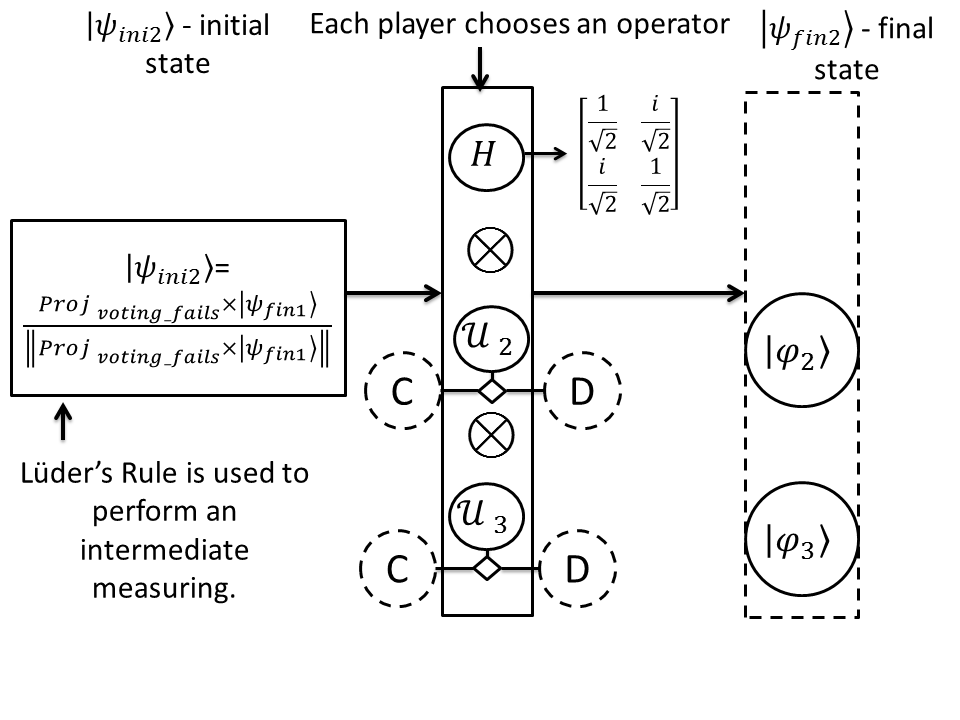
\includegraphics[scale=0.35]{Figures/architecture/esquema/Slide2.png}
\caption{Playing the second round of the Pirate Game with 3 players by performing an intermediate measuring. }
\label{fig:pg_architecture3players_2measure}
\end{figure}

\begin{figure}[h]
\centering 
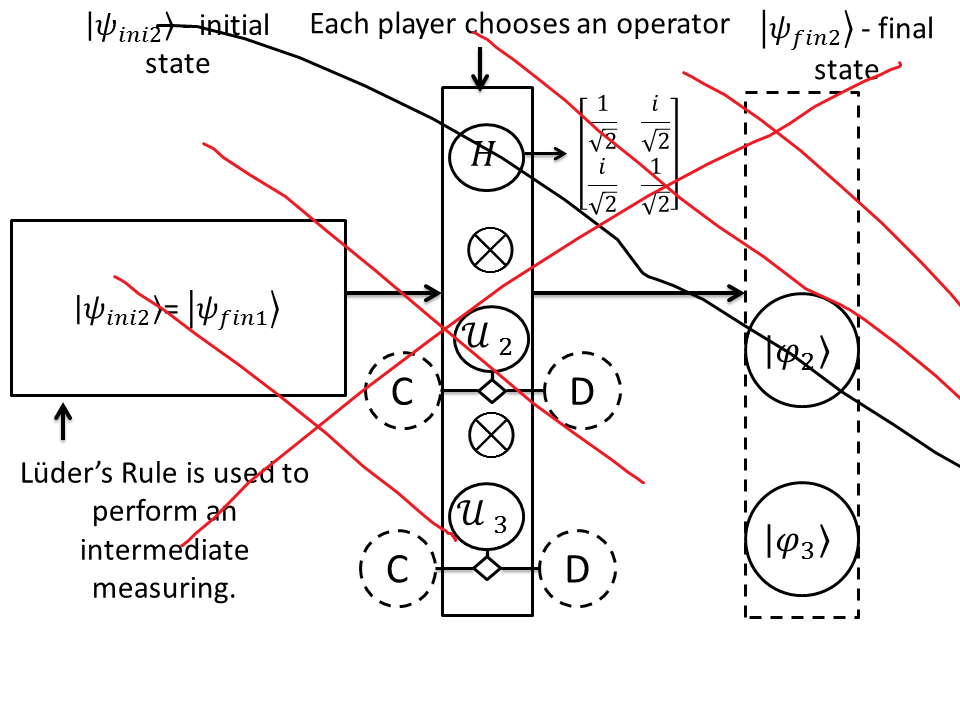
\includegraphics[scale=0.35]{Figures/architecture/esquema/Slide3.png}
\caption{Playing the second round of the Pirate Game with 3 players without performing an intermediate measurement. }
\label{fig:pg_architecture3players_2nomeasure}
\end{figure}

The second stage in the game can be played in one of two ways. Either we perform an intermediate measuring step on the final state from the first round of voting as in Figure \ref{fig:pg_architecture3players_2measure}, or we ``ask'' what are the two player's strategy for this round without informing them of the results in the last round, like in the Figure \ref{fig:pg_architecture3players_2nomeasure}. In the original game the voting results are displayed in between rounds:

\begin{quotation}
If a majority or a tie is reached the goods will be allocated according to the proposal. Otherwise the proposer will be thrown overboard and the next pirate in the hierarchy assumes the place of the captain. 
\end{quotation}

When modelling this problem we want to study if withholding the results in the intermediate step will give way to new strategies.

\begin{figure}[h]
\centering 
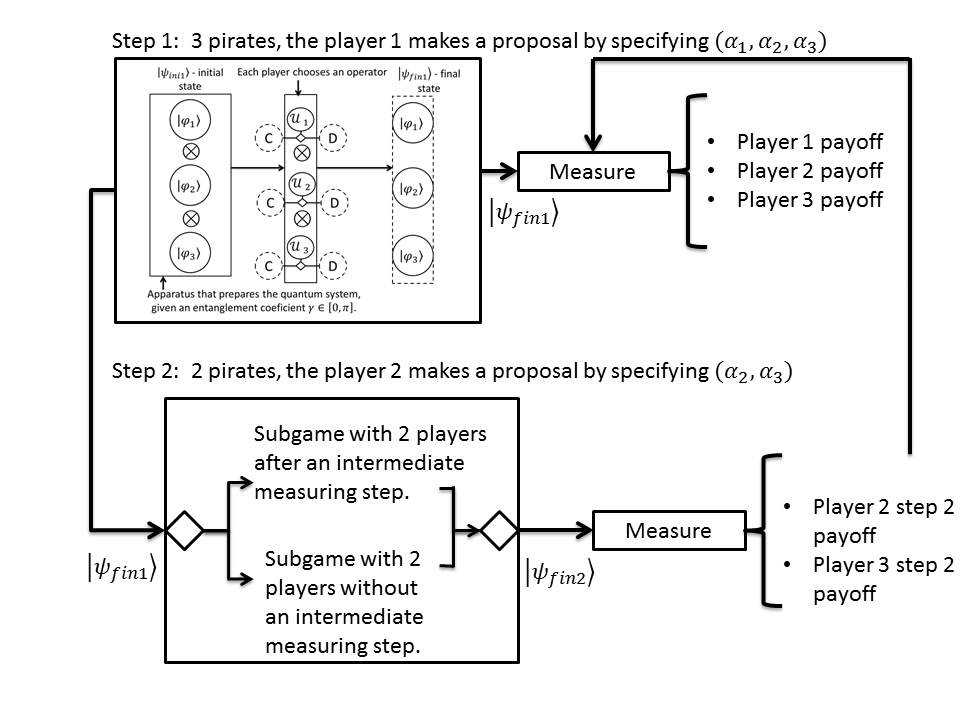
\includegraphics[scale=0.55]{Figures/architecture/esquema/Slide5.png}
\caption{Overal view on the Quantum Pirate Game architecture. }
\label{fig:pg_architecture3players_architecture}
\end{figure}

\subsubsection{Utility}
\label{subsec:pirates_utility}

To build the expected payoff functionals for the three player situation we must take into account the sub-games created when the proposal fail. In Figure \ref{fig:pg_architecturegametree} we can see an extensive form representation of the game.



As defined on Equation \ref{eq:quantum_game_definition_payoff_func},for each player we must specify a utility functional that attributed a real number to the measurement of the projection of a basis in the quantum state that we get after the game. 


This measurement can be understood as a probability of the system collapsing into that state (that derives from the Born Rule, Section \ref{subsubsec:bornrule}).


These utility functions will represent the degree of satisfaction for each pirate after game by atributiong a real number to a measurement performed to the system (as in Equation \ref{eq:quantum_game_definition_payoff_func}, Section \ref{sec:background_quantum_game_theory}). 
The real numbers used convey the logical relations of utility posed by the original problem description. Those numbers will represent the utility associated with the number of coins that a pirate gets, a death penalty, and a small incentive to climb the hierarchy. As each pirate wants to maximize her utility, the Nash equilibrium will be thoroughly used to find the strategies that the pirates will adopt\cite{nash50}\cite{Nash51}.

The number of coins will translate directly the utility associated with getting those coins. For example if a pirate receives 5 gold coins and the proposal is accepted he will get a utility of 5. 

The highest ranking pirate in the hierarchy will be responsible to make a proposal to divide the 100 gold coins. This proposal is modelled as choosing some parameters for the payoff functionals for every player, according to some rules. For the initial step in the game with three pirates these parameters will be $\alpha_{1}, \alpha_{2}, \alpha_{3}$, and they will obey to the Equation \ref{eq:goodss}, where $k$ is the offest of the current captain, and $N$ the number of pirates in the game. 

\begin{equation}
\label{eq:goodss}
\sum_{i=k}^{N}\alpha_{i}=100, \forall i :\alpha_{i}\in\mathbb{N}_{0}
\end{equation}

The most interesting values for $(\alpha_{1}, \alpha_{2}, \alpha_{3})$ will be the allocation that results in a Nash equilibrium in the original Pirate Game $(99, 0, 1)$, and the case where the captain maximizes the number of coins he can get $(100, 0, 0)$. Will the game modelled as a quantum system allow the captain to acquire all the coins?

The proposed goods allocation will be executed if there is a majority (or a tie), in the voting step. A step in the game consists on the highest ranking pirate defining a proposal and the subsequent vote, where all players choose simultaneously an operator. 

If the proposal is rejected the captain will be thrown off board, to account for the fact that this situation is very undesirable for the captain he will receive a negative payoff of $-200$. This value was chosen to be much less than the highest number of coins a pirate could get.

\begin{quotation}
``When the result is indifferent the pirates prefer to throw another pirate overboard and thus climbing in the hierarchy.''
\end{quotation}

This means that the pirates have a small incentive to climb the hierarchy. For example in the three player classical game, the third player, who has the lowest rank, will prefer to defect the initial proposal if the player 1 doesn't give her a coin, even knowing that in the second round the player 2 will be able to keep the 100 coins. We will account for this preference by assigning an expected value of half a coin ($0.5$), to the payoff of the players that will climb on the hierarchy if the voting fails.


We can observe that in Equations \ref{eq:pirates_payoff32} and \ref{eq:pirates_payoff3} that we have two separate groups of outcomes: 
\begin{itemize}
\item Outcomes where the proposal is passed:
\begin{itemize}
\item $\vert CCC\rangle$ or $\vert000\rangle$ (which we measure with $\vert\langle000\vert\psi_{fin}\rangle\vert^{2}$ );
\item $\vert DCC\rangle$ or $\vert100\rangle$;
\item $\vert CDC\rangle$ or $\vert010\rangle$;
\item $\vert CCD\rangle$ or $\vert001\rangle$.
\end{itemize}
\item outcomes where the captain will be eliminated and the remaining players will keep playing:
\begin{itemize}
\item $\vert DDD\rangle$ or $\vert111\rangle$;
\item $\vert DDC\rangle$ or $\vert110\rangle$;
\item $\vert CDD\rangle$ or $\vert011\rangle$;
\item $\vert DCD\rangle$ or $\vert101\rangle$.
\end{itemize}
\end{itemize}



So with $3$ pirates we start with step $1$ (Figure \ref{fig:pg_architecture3players_architecture}), if the voting is rejected we will get to step $2$, where 1 vote is enough to pass a proposal. The final payoff function (for example Equation \ref{eq:pirates_payoff32} for a $3$ player game), will be calculated recursively, the base case being the $2$ player sub-game in a $3$ player system will be Equation \ref{eq:pirates_payoff3}.

 

 \begin{equation}
 \begin{cases}
\begin{split}
E_{11}(\vert\psi_{fin}\rangle, \alpha_{1})=\alpha_{1}\times(\vert\langle000\vert\psi_{fin}\rangle\vert^{2} + \vert\langle100\vert\psi_{fin}\rangle\vert^{2}
+ \vert\langle010\vert\psi_{fin}\rangle\vert^{2}
+ \vert\langle001\vert\psi_{fin}\rangle\vert^{2}
 ) - \\
 - 200\times(\vert\langle111\vert\psi_{fin}\rangle\vert^{2} + \vert\langle110\vert\psi_{fin}\rangle\vert^{2}
+ \vert\langle101\vert\psi_{fin}\rangle\vert^{2}
+ \vert\langle011\vert\psi_{fin}\rangle\vert^{2}
 )
\end{split}
\\
\begin{split}
E_{12}(\vert\psi_{fin}\rangle, \alpha_{2})=\alpha_{2}\times(\vert\langle000\vert\psi_{fin}\rangle\vert^{2} + \vert\langle100\vert\psi_{fin}\rangle\vert^{2}
+ \vert\langle010\vert\psi_{fin}\rangle\vert^{2}
+ \vert\langle001\vert\psi_{fin}\rangle\vert^{2}
 ) - \\
 + (0.5 + E_{22})\times(\vert\langle111\vert\psi_{fin}\rangle\vert^{2} + \vert\langle110\vert\psi_{fin}\rangle\vert^{2}
+ \vert\langle101\vert\psi_{fin}\rangle\vert^{2}
+ \vert\langle011\vert\psi_{fin}\rangle\vert^{2}
 )
\end{split}
\\
\begin{split}
E_{13}(\vert\psi_{fin}\rangle, \alpha_{3})=\alpha_{3}\times(\vert\langle000\vert\psi_{fin}\rangle\vert^{2} + \vert\langle100\vert\psi_{fin}\rangle\vert^{2}
+ \vert\langle010\vert\psi_{fin}\rangle\vert^{2}
+ \vert\langle001\vert\psi_{fin}\rangle\vert^{2}
 ) - \\
 + (0.5 + E_{23})\times(\vert\langle111\vert\psi_{fin}\rangle\vert^{2} + \vert\langle110\vert\psi_{fin}\rangle\vert^{2}
+ \vert\langle101\vert\psi_{fin}\rangle\vert^{2}
+ \vert\langle011\vert\psi_{fin}\rangle\vert^{2}
 )
\end{split}
\end{cases}
\label{eq:pirates_payoff32}
%\caption{Payoff funcionals for the $3$ player pirate game. The payoff function for the non-captain players is recursive because their decision to approve or reject the initial proposal will depend on how much they expect to gain in the next round ($E_{22}$ and $E_{23}$).}
\end{equation}

 \begin{equation}
\begin{cases}
\begin{split}
E_{22}(\vert\psi_{fin2}\rangle, \alpha_{2})=\alpha_{2}\times(\vert\langle000\vert\psi_{fin1}\rangle\vert^{2} + \vert\langle100\vert\psi_{fin1}\rangle\vert^{2}
+ \vert\langle010\vert\psi_{fin1}\rangle\vert^{2}
+ \vert\langle001\vert\psi_{fin1}\rangle\vert^{2}
 ) - \\
 + 0.5\times(\vert\langle111\vert\psi_{fin1}\rangle\vert^{2} + \vert\langle110\vert\psi_{fin1}\rangle\vert^{2}
+ \vert\langle101\vert\psi_{fin1}\rangle\vert^{2}
+ \vert\langle011\vert\psi_{fin1}\rangle\vert^{2}
 )
\end{split}
\\
\begin{split}
E_{23}(\vert\psi_{fin2}\rangle, \alpha_{3})=\alpha_{3}\times(\vert\langle000\vert\psi_{fin1}\rangle\vert^{2} + \vert\langle100\vert\psi_{fin1}\rangle\vert^{2}
+ \vert\langle010\vert\psi_{fin1}\rangle\vert^{2}
+ \vert\langle001\vert\psi_{fin1}\rangle\vert^{2}
 ) - \\
 + 100.5 \times(\vert\langle111\vert\psi_{fin1}\rangle\vert^{2} + \vert\langle110\vert\psi_{fin1}\rangle\vert^{2}
+ \vert\langle101\vert\psi_{fin1}\rangle\vert^{2}
+ \vert\langle011\vert\psi_{fin1}\rangle\vert^{2}
 )
\end{split}
\end{cases}
\label{eq:pirates_payoff3}
%\caption{Second round of a $3$ player game.The $2$ player subgame is the base case for this problem because one vote is enough to pass the proposal.}
\end{equation}


\section{Analysis and Results}
\label{sec:description_3}

%\subsection{$2$ Player Game}
%\label{subsec:2playergame}

\subsection{$3$ Player Game}
\label{subsec:3playergame}

\subsubsection{The captain proposes: $(99, 0, 1)$}
\label{subsubsec:3playergame99}

The outcome $CDC$ with a proposal of $(\alpha_{1}, \alpha_{2}, \alpha_{3}) =(99, 0, 1)$ would represent the Nash Equilibrium of the classic Pirate Game (for $3$ players). 

When the players chose at least $2$ operators $Cooperate$ on the initial proposal the game ends right away, the disentangle operator $\mathcal{J}^{\dagger}$ is applied, and the payoff functionals are calculated given the final state. The final state will be calculated as in Equation \ref{eq:piratas_final_move2_99anal}. 

Tables \ref{tab:3playerCCC99}, \ref{tab:3playerCCD99}, \ref{tab:3playerCDC99}, and \ref{tab:3playerDCC99}present the results for the sittuation described above.

When the first proposal is rejected (more than $1$ player chooses to $Defect$), the second round ensues. We calculate the final state for these states with Equation \ref{eq:piratas_final_move2_99anal1}.

\begin{equation}
\label{eq:piratas_final_move2_99anal}
\vert\psi_{fin}\rangle= \mathcal{J}^{\dagger}\vert\psi_{1}\rangle
\end{equation}

\begin{equation}
\label{eq:piratas_final_move2_99anal1}
\vert\psi_{fin}\rangle= \mathcal{J}^{\dagger}\vert\psi_{2}\rangle
\end{equation}

 
\begin{table}
\begin{center}
\begin{tabular}{cc}
  b)\putindeepbox[7pt]{\includegraphics[scale=0.46]{3Accepted99/CCC.PNG}}
    & b1)\putindeepbox[7pt]{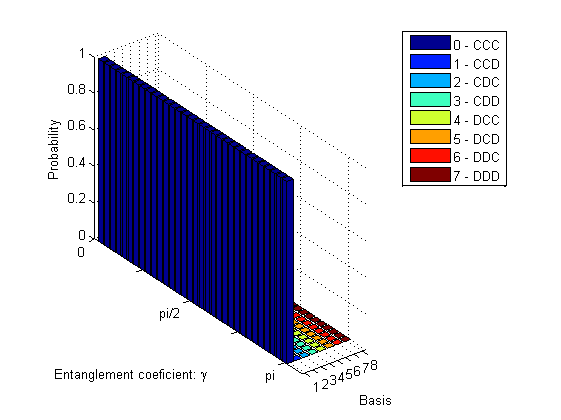
\includegraphics[scale=0.46]{3Accepted99/CCC_1.PNG}} \\
\end{tabular}
\caption{a) Expected utility for $3$ players, where the players will use the $(Cooperate, Cooperate, Cooperate)$ operators. The initial proposal is $(\alpha_{1}, \alpha_{2}, \alpha_{3}) =(99, 0, 1)$. a1) Probability distribution of the final state depending on the entanglement coefitient $\gamma$. }
\label{tab:3playerCCC99}
\end{center}
 \end{table}

\begin{table}
\begin{center}
\begin{tabular}{cc}
  c)\putindeepbox[7pt]{\includegraphics[scale=0.46]{3Accepted99/CCD.PNG}}
    & c1)\putindeepbox[7pt]{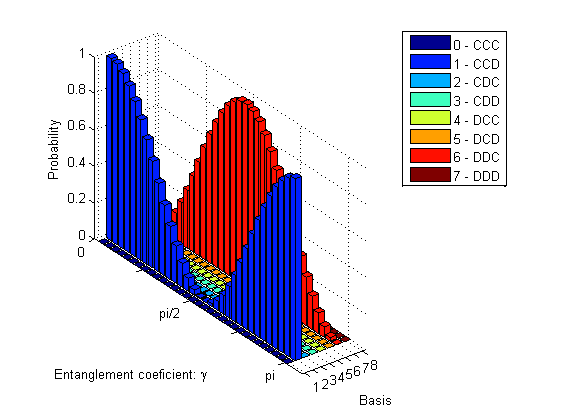
\includegraphics[scale=0.46]{3Accepted99/CCD_1.PNG}} \\
\end{tabular}
\caption{b) Expected utility for $3$ players, where the players will use the $(Cooperate, Cooperate, Defect)$ operators. b1) Probability distruibution of the final state depending on the entanglement coefitient $\gamma$. }
\label{tab:3playerCCD99}
\end{center}
 \end{table}

\begin{table}
\begin{center}
\begin{tabular}{cc}
  a)\putindeepbox[7pt]{\includegraphics[scale=0.46]{3Accepted99/CDC.PNG}}
    & a1)\putindeepbox[7pt]{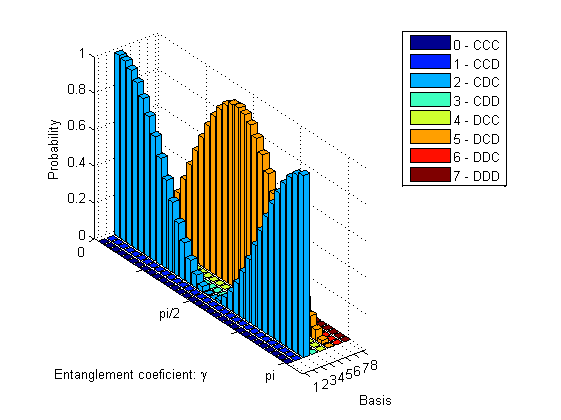
\includegraphics[scale=0.46]{3Accepted99/CDC_1.PNG}} \\
\end{tabular}
\caption{c) Expected utility for $3$ players, where the players will use the $(Cooperate, Defect, Cooperate)$ operators. c1) Probability distribution of the final state depending on the entanglement coefitient $\gamma$. }
\label{tab:3playerCDC99}
\end{center}
 \end{table}

\begin{table}
\begin{center}
\begin{tabular}{cc}
  a)\putindeepbox[7pt]{\includegraphics[scale=0.46]{3Accepted99/DCC.PNG}}
    & a1)\putindeepbox[7pt]{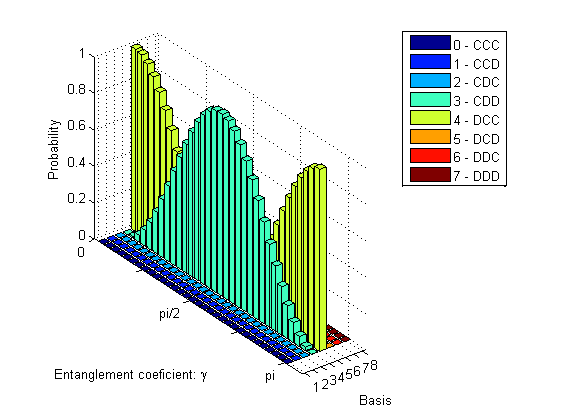
\includegraphics[scale=0.46]{3Accepted99/DCC_1.PNG}} \\
\end{tabular}
\caption{b) Expected utility for $3$ players, where the players will use the $(Defect, Cooperate, Cooperate)$ operators. b1) Probability distrubution of the final state depending on the entanglement coefitient $\gamma$. }
\label{tab:3playerDCC99}
\end{center}
 \end{table}


\subsubsection{The captain proposes: $(100, 0, 0)$}
\label{subsubsec:3playergame100}

Suppose captain is greedy and proposes to get the 100 coins. In the classical Pirate Game this would pose a conflict with his self-preserving needs. 
A pertinent question would be if this Quantum Model of the Pirate Game would allow the first captain to approve an allocation proposal. The initial proposal will be accepted if there is at least $2$ players play $\mathcal{U}_{i}=C$ in a round. In order to answer our question we must analyse the expected utilities for all players when the initial proposal is accepted.

 Our final state will be calculated as in Equation \ref{eq:piratas_final_move2_99anal}.

\begin{table}
\begin{center}
\begin{tabular}{c}
  a)\putindeepbox[7pt]{\includegraphics[scale=0.72]{3Accepted100/CCC.PNG}}
\end{tabular}
\caption{a) Expected utility for $3$ players, where the players will use the $(Cooperate, Cooperate, Cooperate)$ operators. The initial proposal is $(\alpha_{1}, \alpha_{2}, \alpha_{3}) =(100, 0, 0)$. }
\label{tab:3playerCCC100}
\end{center}
 \end{table}

\begin{table}
\begin{center}
\begin{tabular}{c}
  b)\putindeepbox[7pt]{\includegraphics[scale=0.72]{3Accepted100/CCD.PNG}}
\end{tabular}
\caption{b) Expected utility for $3$ players, where the players will use the $(Cooperate, Cooperate, Defect)$ operators. }
\label{tab:3playerCCD100}
\end{center}
 \end{table}

\begin{table}
\begin{center}
\begin{tabular}{c}
  c)\putindeepbox[7pt]{\includegraphics[scale=0.72]{3Accepted100/CDC.PNG}}
   
\end{tabular}
\caption{c) Expected utility for $3$ players, where the players will use the $(Cooperate, Defect, Cooperate)$ operators.}
\label{tab:3playerCDC100}
\end{center}
 \end{table}

\begin{table}
\begin{center}
\begin{tabular}{cc}
  d)\putindeepbox[7pt]{\includegraphics[scale=0.72]{3Accepted100/DCC.PNG}}
\end{tabular}
\caption{d) Expected utility for $3$ players, where the players will use the $(Defect, Cooperate, Cooperate)$ operators. }
\label{tab:3playerDCC100}
\end{center}
 \end{table}


